\documentclass{beamer}

\usepackage{graphicx}
\usepackage{caption}

\begin{document}
	
	\begin{frame}[plain]
		\begin{figure}
			\centering
			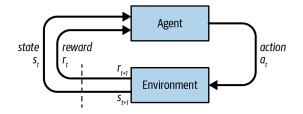
\includegraphics[width=\textwidth,height=0.85\textheight,keepaspectratio]{121.jpg}
			\caption{Reinforcement learning diagram}
		\end{figure}
	\end{frame}
	
	\begin{frame}[plain]
		\begin{figure}
			\centering
			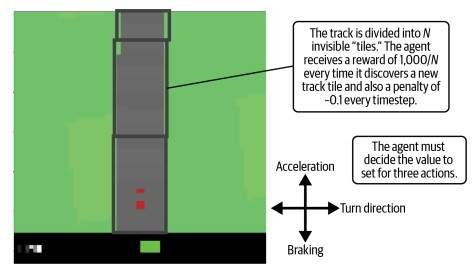
\includegraphics[width=\textwidth,height=0.85\textheight,keepaspectratio]{122.jpg}
			\caption{A graphical representation of one game state in the CarRacing environment}
		\end{figure}
	\end{frame}
	
	
	\begin{frame}[plain]
		\begin{figure}
			\centering
			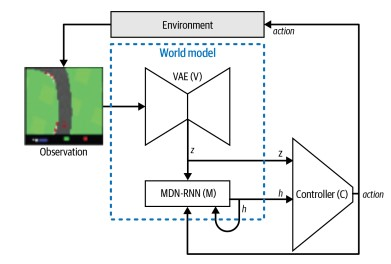
\includegraphics[width=\textwidth,height=0.85\textheight,keepaspectratio]{123.jpg}
			\caption{World model architecture diagram}
		\end{figure}
	\end{frame}
	
	\begin{frame}[plain]
		\begin{figure}
			\centering
			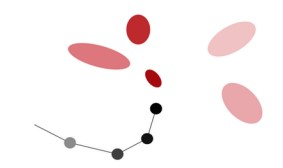
\includegraphics[width=\textwidth,height=0.85\textheight,keepaspectratio]{124.jpg}
			\caption{MDN for handwriting generation}
		\end{figure}
	\end{frame}
	
	\begin{frame}[plain]
		\begin{figure}
			\centering
			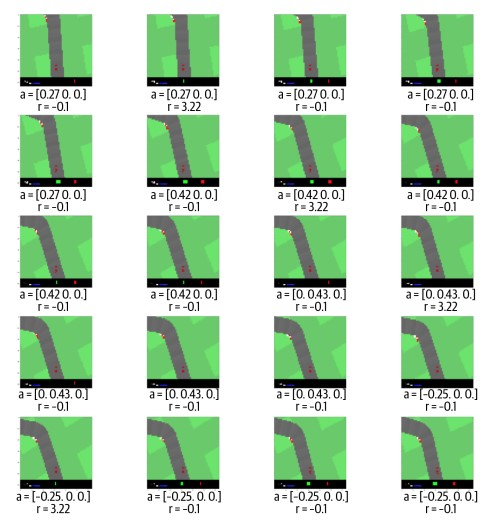
\includegraphics[width=\textwidth,height=0.85\textheight,keepaspectratio]{125.jpg}
			\caption{Frames 40 to 59 of one episode}
		\end{figure}
	\end{frame}
	
	\begin{frame}[plain]
		\begin{figure}
			\centering
			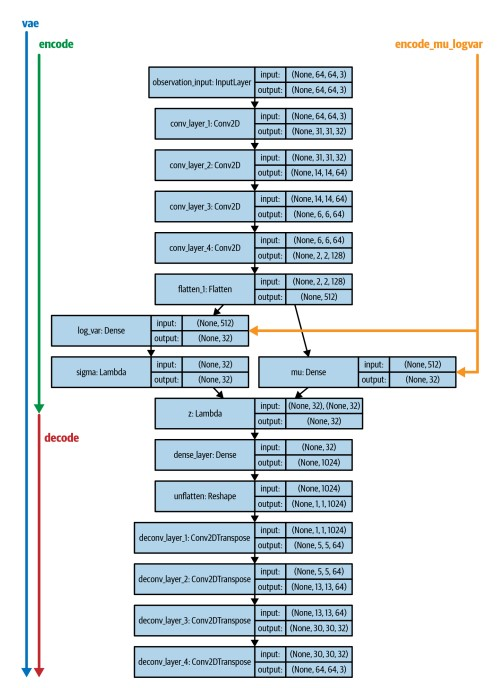
\includegraphics[width=\textwidth,height=0.85\textheight,keepaspectratio]{126.jpg}
			\caption{The VAE architecture from the “World Models” paper}
		\end{figure}
	\end{frame}
	
	\begin{frame}[plain]
		\begin{figure}
			\centering
			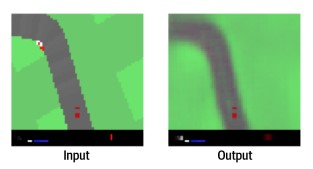
\includegraphics[width=\textwidth,height=0.85\textheight,keepaspectratio]{127.jpg}
			\caption{The input and output from the VAE model}
		\end{figure}
	\end{frame}
	
	\begin{frame}[plain]
		\begin{figure}
			\centering
			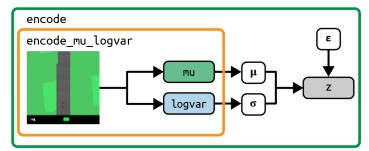
\includegraphics[width=\textwidth,height=0.85\textheight,keepaspectratio]{128.jpg}
			\caption{The output from the encoder models}
		\end{figure}
	\end{frame}
	
	\begin{frame}[plain]
		\begin{figure}
			\centering
			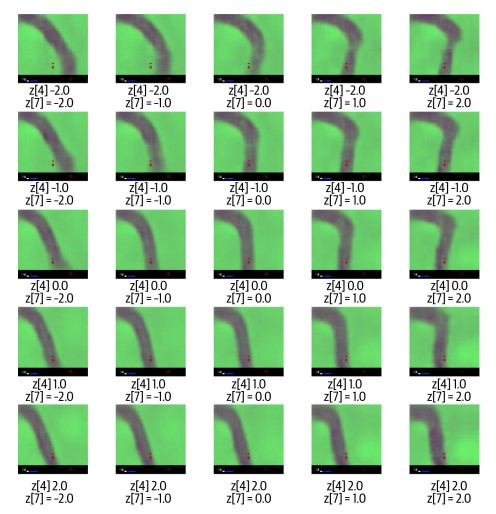
\includegraphics[width=\textwidth,height=0.85\textheight,keepaspectratio]{129.jpg}
			\caption{A linear interpolation of two dimensions of z}
		\end{figure}
	\end{frame}
	
	\begin{frame}[plain]
		\begin{figure}
			\centering
			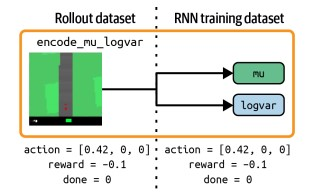
\includegraphics[width=\textwidth,height=0.85\textheight,keepaspectratio]{1210.jpg}
			\caption{Creating the MDN-RNN training dataset}
		\end{figure}
	\end{frame}
	
	\begin{frame}[plain]
		\begin{figure}
			\centering
			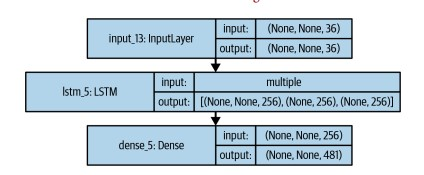
\includegraphics[width=\textwidth,height=0.85\textheight,keepaspectratio]{1211.jpg}
			\caption{The MDN-RNN architecture}
		\end{figure}
	\end{frame}
	
	\begin{frame}[plain]
		\begin{figure}
			\centering
			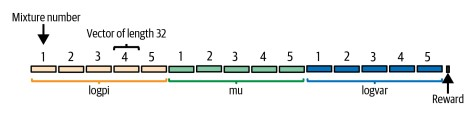
\includegraphics[width=\textwidth,height=0.85\textheight,keepaspectratio]{1212.jpg}
			\caption{The output from the mixture density network}
		\end{figure}
	\end{frame}
	
	\begin{frame}[plain]
		\begin{figure}
			\centering
			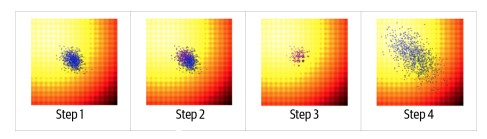
\includegraphics[width=\textwidth,height=0.85\textheight,keepaspectratio]{1213.jpg}
			\caption{One update step from the CMA-ES algorithm}
		\end{figure}
	\end{frame}
	
	\begin{frame}[plain]
		\begin{figure}
			\centering
			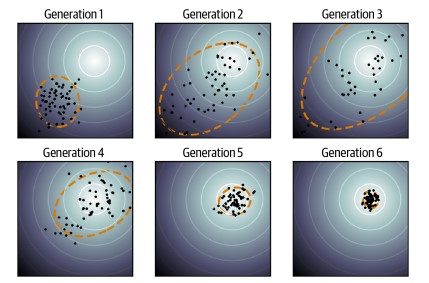
\includegraphics[width=\textwidth,height=0.85\textheight,keepaspectratio]{1214.jpg}
			\caption{CMA-ES}
		\end{figure}
	\end{frame}
	
	\begin{frame}[plain]
		\begin{figure}
			\centering
			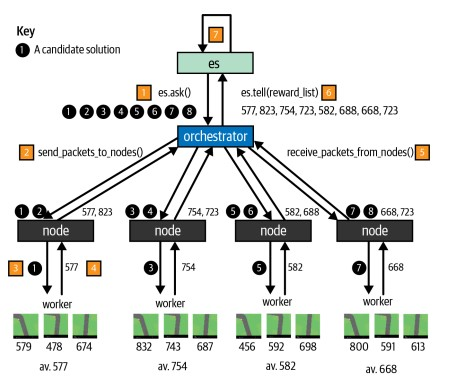
\includegraphics[width=\textwidth,height=0.85\textheight,keepaspectratio]{1215.jpg}
			\caption{Parallelizing CMA-ES—here there is a population size of eight and four
				nodes (so t = 2, the number of trials that each node is responsible for)}
		\end{figure}
	\end{frame}
	
	\begin{frame}[plain]
		\begin{figure}
			\centering
			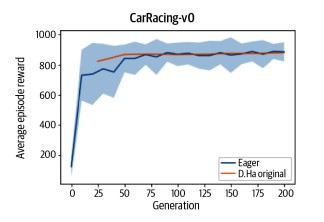
\includegraphics[width=\textwidth,height=0.85\textheight,keepaspectratio]{1216.jpg}
			\caption{Average episode reward of the controller training process, by generation}
		\end{figure}
	\end{frame}
	
	\begin{frame}[plain]
		\begin{figure}
			\centering
			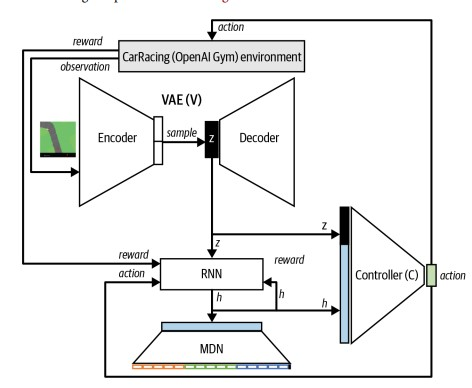
\includegraphics[width=\textwidth,height=0.85\textheight,keepaspectratio]{1217.jpg}
			\caption{Training the controller in the Gym environment}
		\end{figure}
	\end{frame}
	
	\begin{frame}[plain]
		\begin{figure}
			\centering
			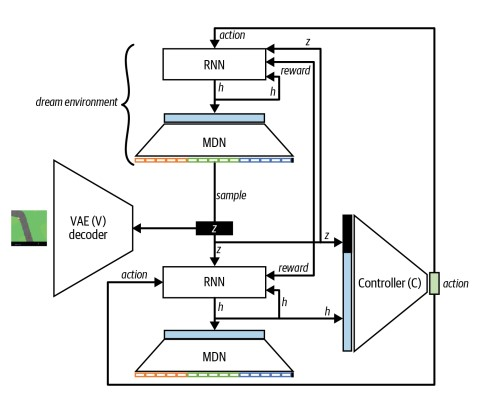
\includegraphics[width=\textwidth,height=0.85\textheight,keepaspectratio]{1218.jpg}
			\caption{Training the controller in the MDN-RNN dream environment}
		\end{figure}
	\end{frame}
	
	\begin{frame}[plain]
		\begin{figure}
			\centering
			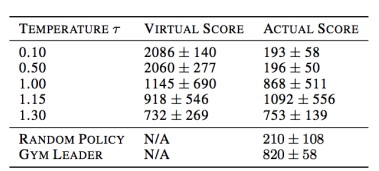
\includegraphics[width=\textwidth,height=0.85\textheight,keepaspectratio]{1219.jpg}
			\caption{Using temperature to control dream environment volatility}
		\end{figure}
	\end{frame}
	
\end{document}